\documentclass[main.tex]{subfiles}

%\externalcitedocument{bibfile}

\begin{document}

\section{Neutrinos Today}

Of the seventeen fundamental particles known to exist, illustrated in Figure~\ref{fig:party}, three are neutrinos. 
This three-neutrino model has been well-established after several decades of study~\cite{PhysRevD.98.030001,Esteban_2019,de_Salas_2018,Capozzi_2016,zboson2006, berns2021recent}.
Despite this success, several anomalies exist in short-baseline neutrino oscillations experiments in $\nu_{\mu}\to\nu_{e}$ appearance~\cite{aguilar2018significant}, reactor neutrino experiments~\cite{mention2011reactor,serebrov2019first}, and in Gallium~\cite{PhysRevC.73.045805,giunti2011statistical}. 
Several of these could be explained by additional oscillations of unknown neutrino mass and flavor eigenstates with eV$^{2}$-scale mass squared differences from the known active states~\cite{abazajian2012light}. 
To be consistent with measurements of Z-boson decay~\cite{zboson2006} any light new flavor state would need to be non weakly-interacting, or ``sterile''. 
One of the simplest models satisfying these criteria is the ``3+1'' light sterile neutrino model in which only a single sterile neutrino is added to the three-neutrino paradigm. 
This introduces a single mass eigenstate $\nu_{4}$ that is sufficiently heavy, compared to the other three, such as to be described by a single mass difference $\Delta m_{41}=m_{4}-m_{1}$. 
Since the states are non-interacting, the most direct way\footnote{Indirect probes of sterile neutrinos are possible through the neutrino effective mass in $0\nu\beta\beta$ decays if the neutrino is Majorana~\cite{HUANG2019114691}} of testing for their existence is through neutrino oscillations. 

Several recent developments have further motivated exploration of the 3+1 sterile neutrino landscape. 
Recent results from MicroBooNE~\cite{microboonecollaboration2021search,microboonecollaboration2021searchmulti} have failed to support the 3+1 explanation of the MiniBoone low-energy excess~\cite{aguilar2018significant}. 
While the implications of this new tension were just starting to be understood~\cite{arguelles2021microboone,denton2021sterile}, the Baksan Experiment on Sterile Transitions (BEST) has instead strongly validated existing anomalies in Gallium short-baseline oscillations experiments, having found strong evidence of sterile neutrino oscillations in $\nu_{e}$ disappearance in excess of $3\sigma$ with a best fit at $\Delta m^{2}=3.3$ eV$^{2}$ and $\sin^{2}2\theta_{14}=0.42$~\cite{barinov2021results, Barinov_2022}. 
Meanwhile Neutrino-4 claims signal at a similar significance at $2.9\sigma$ in $\bar{\nu_{e}}$ disappearance, preferring a 3+1 model with $\Delta m^{2}=7.3$ eV$^{2}$ and $\sin^{2}2\theta_{14}=0.38$~\cite{serebrov2019first}.
By leveraging matter-enhanced oscillations, IceCube has independently observed signal-like evidence at the 90\% confidence level in one of the strongest $\bar{\nu}_{\mu}$ disappearance measurements to date~\cite{Aartsen_2020, Aartsen_2020_prd}.
These results complicate matters as they strongly refute previous solutions to the anomalies in MiniBooNE and LSND~\cite{Athanassopoulos_1998}, and other constraints around 1~eV$^{2}$~\cite{kopp2013sterile, Cirelli:2004cz, abazajian2012light, Gariazzo:2017fdh, Dentler:2017tkw, Diaz:2019fwt}.
These previous IceCube $\nu_{\mu}$ disappearance results, however, conservatively assumed $\theta_{14}=\theta_{34}=0$. 
And so strong motivations are abundant to expand these previous IceCube analyses in a widened search, taking advantage of newer event morphologies, to study signatures we might expect given the results from BEST. 

First, however, we begin with a review of the physics relevant to neutrinos.

\begin{figure}
    \centering
    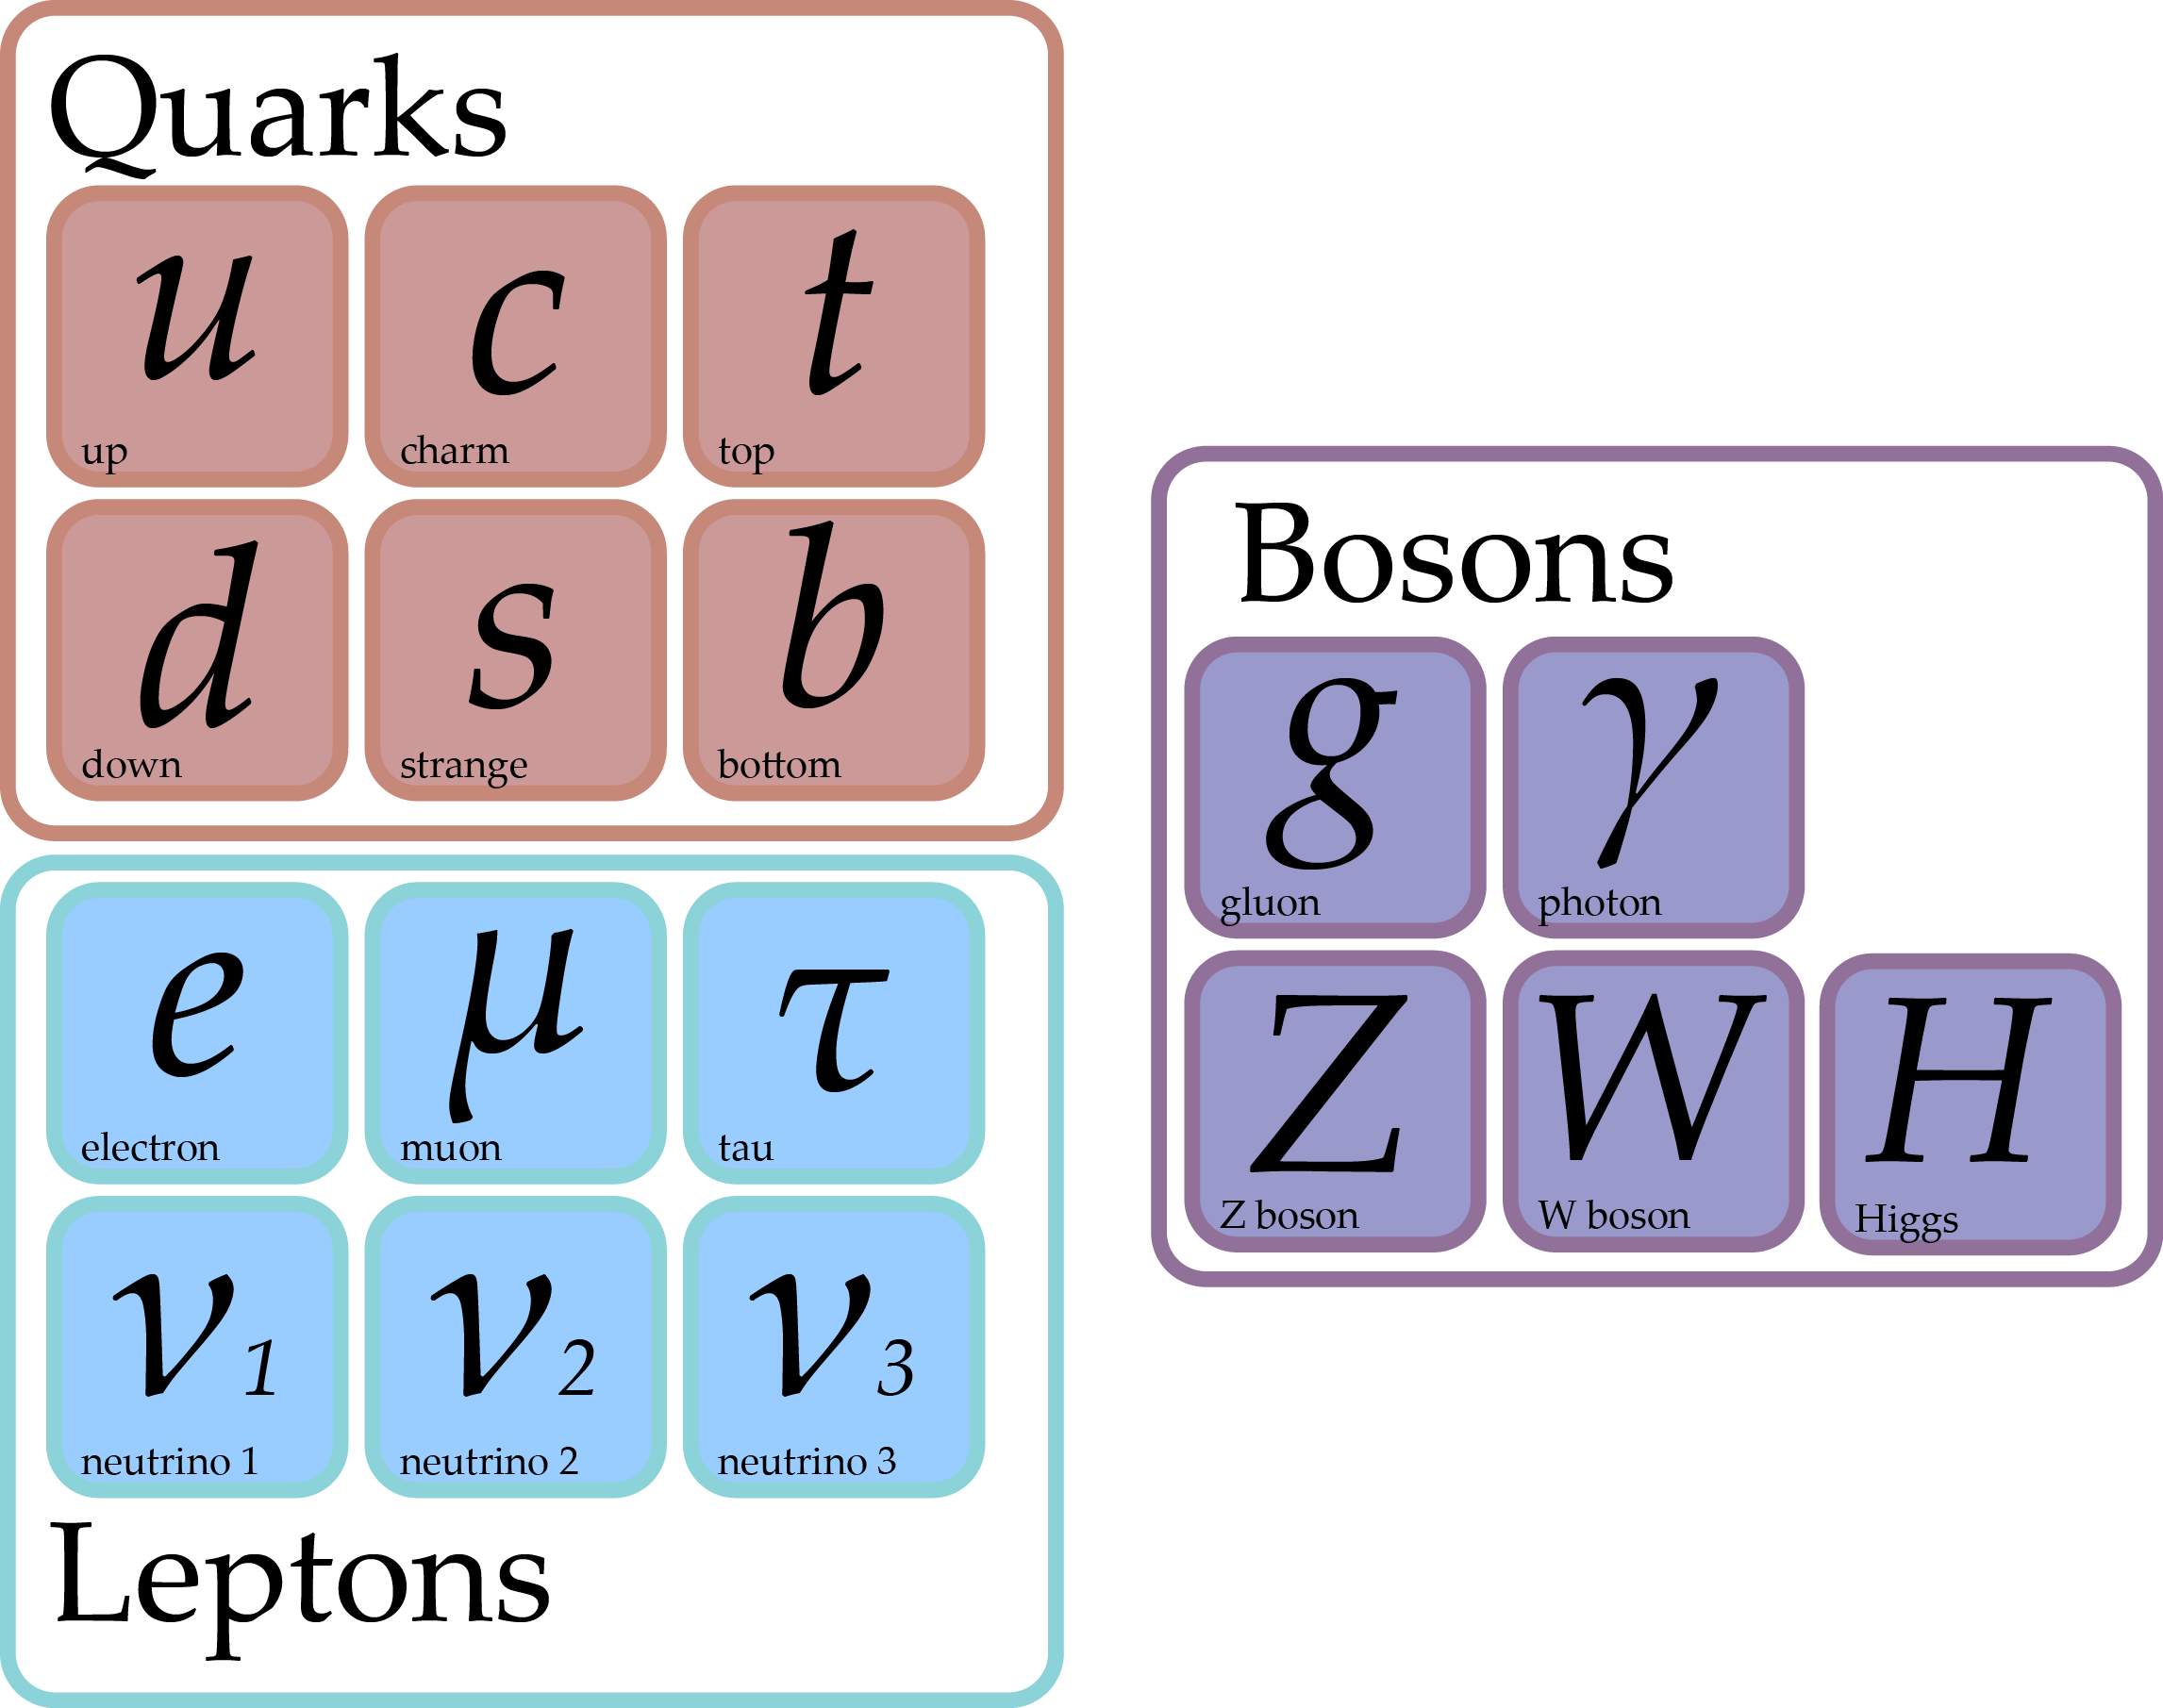
\includegraphics[width=0.8\linewidth]{figures/particles.png}
    \caption{A table of the seventeen fundamental particles. The mass eigenstates for the fermions are shown.}\label{fig:party}
\end{figure}

\section{Neutrino oscillations}
\index{neutrino!oscillations}

The weak interaction couples left-handed neutrinos and charged leptons in SU(2) doublets,
\begin{align}
&\left(\begin{array}{c} \nu_{e} \\ e^{-} \end{array}\right) & &\left(\begin{array}{c} \nu_{\mu} \\ \mu^{-} \end{array}\right) & &\left(\begin{array}{c} \nu_{\tau} \\ \tau^{-} \end{array}\right).
\end{align}
As a consequence, neutrinos can only be produced in one of these three flavor eigenstates.
Similar to in the quark sector, the neutrino flavor eigenstates can be expressed as linear superpositions of the mass eigenstates, which are related to one another by the unitary Pontecorvo-Maki-Nakagawa-Sakata (PMNS) matrix in the standard $3\nu$ model
\begin{equation}
    U_{\text{PMNS}} = \left(\begin{array}{ccc} U_{e1} & U_{e2} & U_{e3} \\ U_{\mu 1} & U_{\mu 2} & U_{\mu 3} \\ U_{\tau 1} & U_{\tau 2} & U_{\tau 3} \end{array}\right).
\end{equation}
And so the mass-basis is related to the flavor basis as
\begin{equation}
    \left(\begin{array}{ccc} \nu_{e} & \nu_{\mu} & \nu_{\tau} \end{array}\right)  = \left(\begin{array}{ccc} U_{e1} & U_{e2} & U_{e3} \\ U_{\mu 1} & U_{\mu 2} & U_{\mu 3} \\ U_{\tau 1} & U_{\tau 2} & U_{\tau 3} \end{array}\right) \left(\begin{array}{c} \nu_{1} \\ \nu_{2} \\ \nu_{3} \end{array}\right),
\end{equation}
where $\nu_{i}$, $i\in\left(1,2,3\right)$ is in the mass basis and $i\in\left(e,\mu\tau\right)$ is in the flavor basis. 
We can, in general then, express a stationary neutrino state in the flavor basis in terms of the mass basis. 
First, let us consider two neutrino oscillations, where a generic SU(2) matrix can be written as 
\begin{equation}
    U_{2d}=\left(\begin{array}{cc} \cos\theta & \sin\theta \\ -\sin\theta & \cos\theta \end{array}\right)
\end{equation}
where $\theta$ is some real-valued angle describing a rotation from one basis to the other. So we can write an initial $\ket{\nu_{e}}$ state as 
\begin{equation}\label{eq:nunu}
    \ket{\nu_{e}} = \cos\theta \ket{\nu_{1}} + \sin\theta \ket{\nu_{2}}.
\end{equation}
A time-evolved neutrino state will be one solving the time-dependent Schr\"odinger Equation,
\begin{equation}
    i\dfrac{\partial}{\partial t} \ket{\nu_{i} (t)} = \bvec{H}_{\nu}\ket{\nu_{i}(t)},
\end{equation}
which we can do with a stationary state solution
\begin{equation}\label{eq:stationary}
    \ket{\nu_{i} (t)}  =  e^{-iEt} \ket{\nu_{i} (0)}.
\end{equation}
Neutrinos are known to have very small masses~\cite{KATRIN:2021uub}, and so we expand out an expression of the four-momentum energy and cut off any terms with $\mathcal{O}(>m^{2})$. 
\begin{align}
    E_{i} &= \sqrt{p^{2}c^{2} + m_{i}^{2}c^{4}} \\
    &\approxeq pc + \dfrac{m_{i}^{2}c^{4}}{2E}
\end{align}
The stationary state solution Equation~\eqref{eq:stationary} becomes, using $t=L/c$ and $c=1$ 
\begin{equation}
    \ket{\nu_{i} (t)}  =  e^{-ipt}e^{ -im_{i}^{2}L/2E}\ket{\nu_{i} (0)}
\end{equation}
and for the state described in Equation~\eqref{eq:nunu},
\begin{equation}
    \ket{\nu_{e}(t)} = e^{-ipt}e^{ -im_{1}^{2}L/2E} \cos\theta \ket{\nu_{1}}  + e^{-ipt}e^{ -im_{2}^{2}L/2E} \sin\theta \ket{\nu_{2}}.
\end{equation}
Considering the muon flavor state expressed in the mass basis,
\begin{equation}
    \bra{\nu_{\mu}} = -\sin\theta\bra{\nu_{1}} + \cos\theta\bra{\nu_{2}},
\end{equation}
the oscillations probabilities can be calculated by projecting the final considered state onto the evolved state.
\begin{align}
    \braket{\nu_{\mu} | \nu_{e}(t)} &= -e^{-ipt}e^{ -im_{1}^{2}L/2E} \cos\theta\sin\theta  + e^{-ipt}e^{ -im_{2}^{2}L/2E} \sin\theta\cos\theta \\
    \braket{\nu_{\mu} | \nu_{e}(t)} &= \tfrac{1}{2}e^{-ipt}\left[e^{ -im_{2}^{2}L/2E} - e^{ -im_{1}^{2}L/2E}\right] \sin 2\theta
\end{align}
To calculate actual transmission probabilities, we need the conjugate-square of this, $P_{e\mu} \equiv \left|\braket{\nu_{\mu}|\nu_{e}(t)}\right|^{2}$. While the phase term, $e^{-ipt}$, cancels we are left with 
\begin{align}
    \braket{\nu_{\mu} | \nu_{e}(t)} &=\tfrac{1}{4} \left[e^{ -im_{2}^{2}L/2E} - e^{ -im_{1}^{2}L/2E}\right]\left[e^{ im_{2}^{2}L/2E} - e^{ im_{1}^{2}L/2E}\right] \sin^{2} 2\theta \\
    \braket{\nu_{\mu} | \nu_{e}(t)} &=\tfrac{1}{4}\left[1 - e^{-i\Delta m_{21}^{2}L/2E}- e^{i\Delta m_{21}^{2}L/2E}  +1\right]\sin^{2} 2\theta\\
    \braket{\nu_{\mu} | \nu_{e}(t)} &=\tfrac{1}{4}\left[2- 2\cos\left( \Delta m_{21}^{2}L/2E\right) \right]\sin^{2} 2\theta \\
    \braket{\nu_{\mu} | \nu_{e}(t)} &=\left[\dfrac{1-\cos\left( 2\Delta m_{21}^{2}L/4E\right)}{2} \right]\sin^{2} 2\theta \\
    \braket{\nu_{\mu} | \nu_{e}(t)} &=\sin^{2}\left( \dfrac{\Delta m_{21}^{2}L}{4E}\right) \sin^{2} 2\theta
\end{align}

Neutrino oscillation probabilities are dependent not on the mass of the neutrino eigenstates, but the differences of square of the masses over which oscillations are considered.
Through oscillations, we can only measure the absolute of the difference of the masses, and so the ordering of the masses is invisible to neutrino oscillations. 
Since oscillations today are well-established, at minimum two of the neutrino masses must be non-zero. 
Oscillations will also depend on the energy $E$ of the neutrinos involved and the baseline $L$ over which they travel. 

For oscillations over a fixed $L/E$ baseline, the mass-squared splitting will affect the frequency of the neutrino oscillations and the elements in the neutrino mixing matrix will affect the amplitudes of the oscillations. \index{neutrino!baseline}
A toy-model example is shown in Figure~\ref{fig:toy_osc}, where an initial $\nu_{\mu}$ flux is propagated over a fixed baseline. 
A varying amount of the initial flux is expected to oscillate to $\nu_{e}$ as a function of energy. 

\begin{figure}
    \centering
    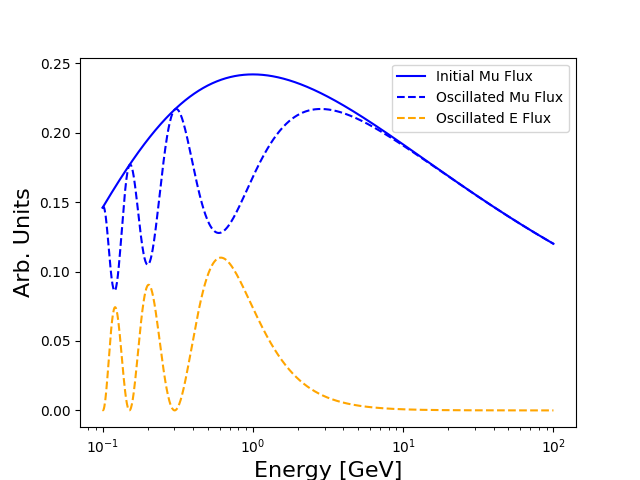
\includegraphics[width=0.6\linewidth]{figures/oscillations_example.png}
    \caption{A toy 2-neutrino oscillations example. The initial flux is shown as a solid blue line, and the propagated fluxes are shown as dashed lines in orange and blue.}\label{fig:toy_osc}
\end{figure}

We next consider the general case of a neutrino initially in the electron-flavor neutrino state. 
\begin{equation}\label{eq:three}
    \ket{\nu_{e}} =\sum\limits_{j} U_{ej} \ket{\nu_{j}} 
\end{equation}
Much like before we evolve an arbitrary stationary state
\begin{equation}
    \ket{\nu_{j} (t)}  = e^{-ipt}e^{ -m_{j}^{2}L/2E}\ket{\nu_{j} (0)}
\end{equation}
such that Equation~\eqref{eq:three} becomes
\begin{equation}
    \ket{\nu_{e}(t)} = \sum\limits_{j} U_{ej} e^{-ipt}e^{ -m_{j}^{2}L/2E}\ket{\nu_{j} (0)}.
\end{equation}
Again, we consider the probability of measuring the neutrino in the muon flavor state some time $t$ after preparing it the electron flavor state. 
\begin{equation}
    \braket{\nu_{\mu} | \nu_{e}(t)} = e^{-ipt} \sum\limits_{j} U_{\mu j}^{*}U_{ej} e^{ -m_{j}^{2}L/2E}
\end{equation}
We need the conjugate-square of this, $P_{e\mu} \equiv \left|\braket{\nu_{\mu}|\nu_{e}(t)}\right|^{2}$.
\begin{equation}\begin{split}
P_{\mu e}&= \sum\limits_{i}\left[\left|U_{\mu i}\right|^{2}\left|U_{e i}\right|^{2} \right.\\
&\hspace{1cm} + 2\sum\limits_{i>j}U_{\mu i}^{*}U_{e i}U_{\mu j}U_{e j}^{*}\left.e^{-i\Delta m_{ij}^{2}L/2E} \right]
\end{split}\end{equation} 
Using the sinusoidal form of the exponential, we can write this in other components 
\begin{equation}\begin{split}
    P_{\mu e}&= \sum\limits_{i}\left[\left|U_{\mu i}\right|^{2}\left|U_{e i}\right|^{2} \right.\\
    &\hspace{1cm} -2\sum\limits_{i>j} \Re(U_{\mu i}^{*}U_{e i}U_{\mu j}U_{e j}^{*})\cos\left(\Delta m_{ij}^{2}L/2E \right) \\
    &\hspace{1cm} -2\sum\limits_{i>j}\Im(U_{\mu i}^{*}U_{e i}U_{\mu j}U_{e j}^{*})\sin\left(\Delta m_{ij}^{2}L/2E \right)
\end{split}\end{equation} 

\iffalse
\subsection{Unitary Matrix Construction for SU(N)}

For larger number of Dirac neutrinos, some of which may be sterile, consider that the $3\times 3$ PMNS matrix is embedded in a larger, unitary, $N\times N$ mixing matrix.
In these cases we construct arbitrary $U\in SU(N)$ as a product of complex rotations parametrized by angles $\theta_{ij}$ and phases $\delta_{ij}$, 
\begin{equation}
    U(\theta_{ij}, \delta_{ij}) = R_{N-1,N}R_{N-2,N}\ldots R_{45}R_{34}R_{24}R_{15}R_{34}R_{24}R_{14}R_{23}R_{13}R_{12}
\end{equation}
% as discussed in Ref~\cite{Arguelles:2020hss}
\fi

\section{Neutrinos and Matter}

%\subsection{Neutrino Interactions}
%\index{neutrino!interactions}
%Discuss neutrino interactions at medium to high energies. Deep Inelastic Scattering

\subsection{Matter Effects on Neutrino Oscillations}
\index{neutrino!matter effect}
Although neutrino-anything cross-sections are small compared to all other standard-model interactions, neutrinos at higher energies\footnote{seen to be relevant in IceCube at energies above a few GeV} passing through a large amount of media can result in a measureable effect on the neutrino flux. 
The neutrinos experience coherent forward elastic scattering with the electrons and nucleons composing the medium through which they propagate. Although all three neutrinos can scatter via Z$^{0}$ boson exchange with nucleons; only $\nu_{e}$ can scatter via the exchange of W$^{\pm}$ and Z$^{0}$ with electrons. 
The consequence of these interactions is that neutrinos behave as if they had slightly different masses, which are referred to as effective masses, and so their oscillations are impacted.  
The mass-modification is parametrized through a weak-field effect from the $Z^{0}$ and $W^{\pm}$ on the neutrino flavor state $\nu_{i}$, which we first write out as
\begin{align} 
    V_{\nu_{i}, e}^{Z^{0}+W^{\pm}} &= -\dfrac{\sqrt{2}}{2}G_{F} N_{e} + \sqrt{2}G_{F}N_{e}  & V_{\nu_{i}, n}^{Z^{0}} &= -\dfrac{\sqrt{2}}{2}G_{F} N_{n} & V_{\nu_{i}, p}^{Z^{0}} &= \dfrac{\sqrt{2}}{2}G_{F} N_{p}
\end{align}
where $G_{F}$ is the Fermi constant and $N_{\alpha}$ is the number density of particle $\alpha$ in the medium. 
If we assume similar numbers of protons and neutrons in a medium the effects of nucleons cancel for each neutrino flavor. 
The resulting weak-field effects, per-flavor, are
\begin{align} \label{eq:matter_weak}
    V_{\nu_{e}}^{Z^{0}+W^{\pm}} &= \dfrac{\sqrt{2}}{2}G_{F} N_{e}  & V_{\nu_{\mu}}^{Z^{0}} &= -\dfrac{\sqrt{2}}{2}G_{F} N_{e} & V_{\nu_{\tau}}^{Z^{0}} &= -\dfrac{\sqrt{2}}{2}G_{F} N_{e}
\end{align}
Differences in the propagation of the different flavors will appear due to a difference in the weak-field potential. 
Since there are only two unique terms, it follows that 
\begin{equation}
    V \equiv V_{\nu_{e}}^{Z^{0}+W^{\pm}} -  V_{\nu_{\mu}}^{Z^{0}}  =  V_{\nu_{e}}^{Z^{0}+W^{\pm}} -  V_{\nu_{\tau}}^{Z^{0}}   = \sqrt{2} G_{F} N_{e}
\end{equation}
We now define a function $V(\vec{x})\equiv  \sqrt{2} G_{F} N_{e}(\vec{x})$ that depends on the electron number-density at arbitrary position $\vec{x}$.  
Since the electron flavor is the only one with a unique matter-effect, the potential difference that could modify neutrino oscillations goes like 
\begin{equation}
    V = V(x)\left(\begin{array}{ccc} 1&0&0\\0&0&0 \\0&0&0 \end{array}\right) 
\end{equation}

From here, we use the small-mass approximation of the neutrino mass
\begin{align} 
    \braket{\nu_{\alpha} | H_{vac} | \nu_{\beta} } &= \braket{ \sum_{i} U_{\alpha i} \nu_{i} \middle| H_{vac} \middle| \sum_{j} U_{\beta j}^{*}\nu_{j}}  \\
    &=  \sum\limits_{j} U_{\alpha j} U^{*}_{e\beta}\left( p + \dfrac{m_{j}^{2}}{2E} \right)
\end{align}
As in the case of vacuum oscillations, it is the relative phases of the mass eigenstate wave packets that contribute to the interference in the flavor basis. 
The \textit{difference} in the energies for the different mass states is what gives rise to neutrino oscillations, so we can equivalently express each of the masses as differences from $m_{1}^{2}$ 
\begin{align}
    H_{\alpha \beta, vac } &= \sum\limits_{j} U_{\alpha j} U^{*}_{\alpha j} \Delta m^{2}_{j1}\\
    H_{vac }&= \dfrac{1}{2E} U\left(\begin{array}{ccc} 0 & 0 & 0 \\ 0 & \Delta m_{21}^{2} & 0 \\ 0 & 0 & \Delta m_{31}^{2} \end{array}\right)U^{\dag}. \label{eq:hamy}
\end{align}

And so we can construct a modified Hamiltonian with the matter contribution 
\begin{equation}
    H_{tot }= \dfrac{1}{2E} \left[ U\left(\begin{array}{ccc} 0 & 0 & 0 \\ 0 & \Delta m_{21}^{2} & 0 \\ 0 & 0 & \Delta m_{31}^{2} \end{array}\right)U^{\dag} + V(x)\left(\begin{array}{ccc} 1&0&0\\0&0&0 \\0&0&0 \end{array}\right)  \right]
\end{equation}

A common tactic for working with this modified Hamiltonian is in the diagonal basis, where the new diagonal elements are treated as \textit{effective} mass eigenstates. 


\subsection{MSW Effect}


The Mikheyev-Smirnov-Wolfenstein (MSW) is a neutrino matter effect effecting neutrino oscillations in media of varying density. 
First, we re-write Equation~\eqref{eq:hamy} in the two neutrino-case. 
\begin{align}
    H_{vac} &= \dfrac{1}{2E}\left(\begin{array}{cc}\cos\theta &\sin\theta \\ -\sin\theta & \cos\theta\end{array}\right)\left(\begin{array}{cc}0 & 0 \\ 0 & \Delta m^{2}\end{array}\right) \left(\begin{array}{cc}\cos\theta &-\sin\theta \\ \sin\theta & \cos\theta\end{array}\right) \\
    &= \dfrac{\Delta m^{2}}{2E}\left(\begin{array}{cc} -\sin^{2}\theta & \cos\theta\sin\theta \\ -\cos\theta \sin\theta & \cos^{2}\theta\end{array}\right)\\
    &= \dfrac{\Delta m^{2}}{4E}\left(\begin{array}{cc} -2\sin^{2}\theta & \sin 2\theta \\ -\sin 2\theta & 2\cos^{2}\theta\end{array}\right)
\end{align}
We can subtract an identity from this since its the relative energy of eigenstates that are important for oscillations,
\begin{align}
    H_{vac}  &= \dfrac{\Delta m^{2}}{4E}\left(\begin{array}{cc} -2\sin^{2}\theta-1 & \sin 2\theta \\ \sin 2\theta & 2\cos^{2}\theta -1\end{array}\right),\\
    H_{vac} &= \dfrac{\Delta m^{2}}{4E}\left(\begin{array}{cc} -\cos 2\theta & \sin 2\theta \\ \sin 2\theta & \cos 2\theta \end{array}\right). \label{eq:vacuum_msw}
\end{align}
When adding in matter-effects, we refer to Equation~\eqref{eq:matter_weak},
\begin{align}
    H_{matter} &= \left(\begin{array}{cc} \tfrac{\sqrt{2}G_{F}N_{e}}{2} & 0 \\ 0 & -\tfrac{\sqrt{2}G_{F}N_{e}}{2} \end{array}\right)\\
    H_{matter} &= \dfrac{\Delta m^{2}}{4E}\left(\begin{array}{cc} \tfrac{2\sqrt{2}G_{F}N_{e}E}{\Delta m^{2}} & 0 \\ 0 & - \tfrac{2\sqrt{2}G_{F}N_{e}E}{\Delta m^{2}} \end{array}\right) \label{eq:matter_only}
\end{align}
and we construct the full Hamiltonian by combining Equations~\eqref{eq:vacuum_msw} and~\eqref{eq:matter_weak}:
\begin{align}\label{eq:hamil_msq}
    H_{tot} &= \dfrac{\Delta m^{2}}{4E}\left(\begin{array}{cc} -(\cos 2\theta - A) & \sin 2\theta \\ \sin 2\theta & \cos 2\theta - A\end{array}\right) & A&= \dfrac{2\sqrt{2} G_{F} N_{e}E}{\Delta m^{2}}.
\end{align}
We can then define an effective mass difference as 
\begin{equation}\label{eq:mass_m}
    \Delta m_{M}^{2} = \Delta m^{2}\sqrt{\sin^{2}2\theta + (\cos 2\theta - A)^{2}}
\end{equation}
and an effecting mixing amplitude as 
\begin{equation}\label{eq:mass_th}
    \sin^{2} 2\theta_{M} = \dfrac{\sin^{2} 2\theta}{\sin^{2} 2\theta + (\cos 2\theta + A)^{2}}.
\end{equation}
Using these, the matter-Hamiltonian of Eq~\eqref{eq:hamil_msq} can be written as 
\begin{equation}\label{eq:wolfwolf}
    H_{tot} = \dfrac{\Delta m_{M}^{2}}{4E}\left(\begin{array}{cc} -\cos 2\theta_{M} & \sin 2\theta_{M} \\ \sin 2\theta_{M} & \cos 2\theta_{M} \end{array} \right).
\end{equation}
As can be seen, as $A\to 0$ Equations~\ref{eq:mass_m} and~\ref{eq:mass_th} yield the original vacuum forms, and so Equation~\ref{eq:wolfwolf} would also predict vacuum oscillations in the absence of matter. 
$A$ itself is also now seen to depend upon the on the sign of the difference of the squares of the mass: in the presence of matter neutrino oscillations can be used to directly probe the neutrino mass ordering. 

\subsection{3+1 Neutrino Oscillations}

Including a fourth, sterile, neutrino flavor and mass eigenstate expands the normal PMNS matrix to SU(4). 
To describe the new SU(4) mixing matrix uniquely, three new mixing angles ($\theta_{14}$, $\theta_{24}$, and $\theta_{34}$) and two new CP-violating phases ($\delta_{14}$ and $\delta_{24}$) are required. 
While this leads to the aforementioned short-baseline neutrino oscillations needed to explain extant oscillation anomalies, it also will yield novel effects in the presence of matter~\cite{Akhmedov:1988kd,KRASTEV1989341,Chizhov:1998ug, Chizhov_1999, Akhmedov_2000}.

For eV-scale sterile neutrino models, the mass difference between the new $\nu_{4}$ and othe mass states are essentially degenerate; we can sufficiently describe the new state using only a single new mass difference $\Delta m_{41} = m_{4}-m_{1}$. 
MSW matter effects would also yield a near complete disappearance of TeV-energy muon anti-neutrinos passing through the Earth's core~\cite{Nunokawa:2003ep, Petcov:2016iiu, Choubey:2007ji, Barger:2011rc, Esmaili:2012nz, esmaili2013restricting, Lindner:2015iaa}, as shown in Figure~\ref{fig:sterile_osc_sig}.
This is of particular interest to large-volume \v{C}erenkov neutrino observatories, like the IceCube Neutrino Observatory, which have high event rates for up-going muon neutrino events. 
Recent results from IceCube searching for such a signature have already found signal-like results with closed contours at the 90\% confidence level and a best fit point at $\sin^2 2\theta_{24}\sim0.1$ and $\Delta m^2_{41}=4.5\text{ eV}^2$~\cite{Aartsen_2020, Aartsen_2020_prd}. 
Despite the signal-like results, the measurement is also in tension with the LSND~\cite{Athanassopoulos_1998}, MiniBooNE, and other constraints for values of $\Delta m_{41}^{2}$ of around 1eV$^{2}$~\cite{kopp2013sterile, Cirelli:2004cz, abazajian2012light, Gariazzo:2017fdh, Dentler:2017tkw, Diaz:2019fwt}.

\begin{figure}
    \centering
    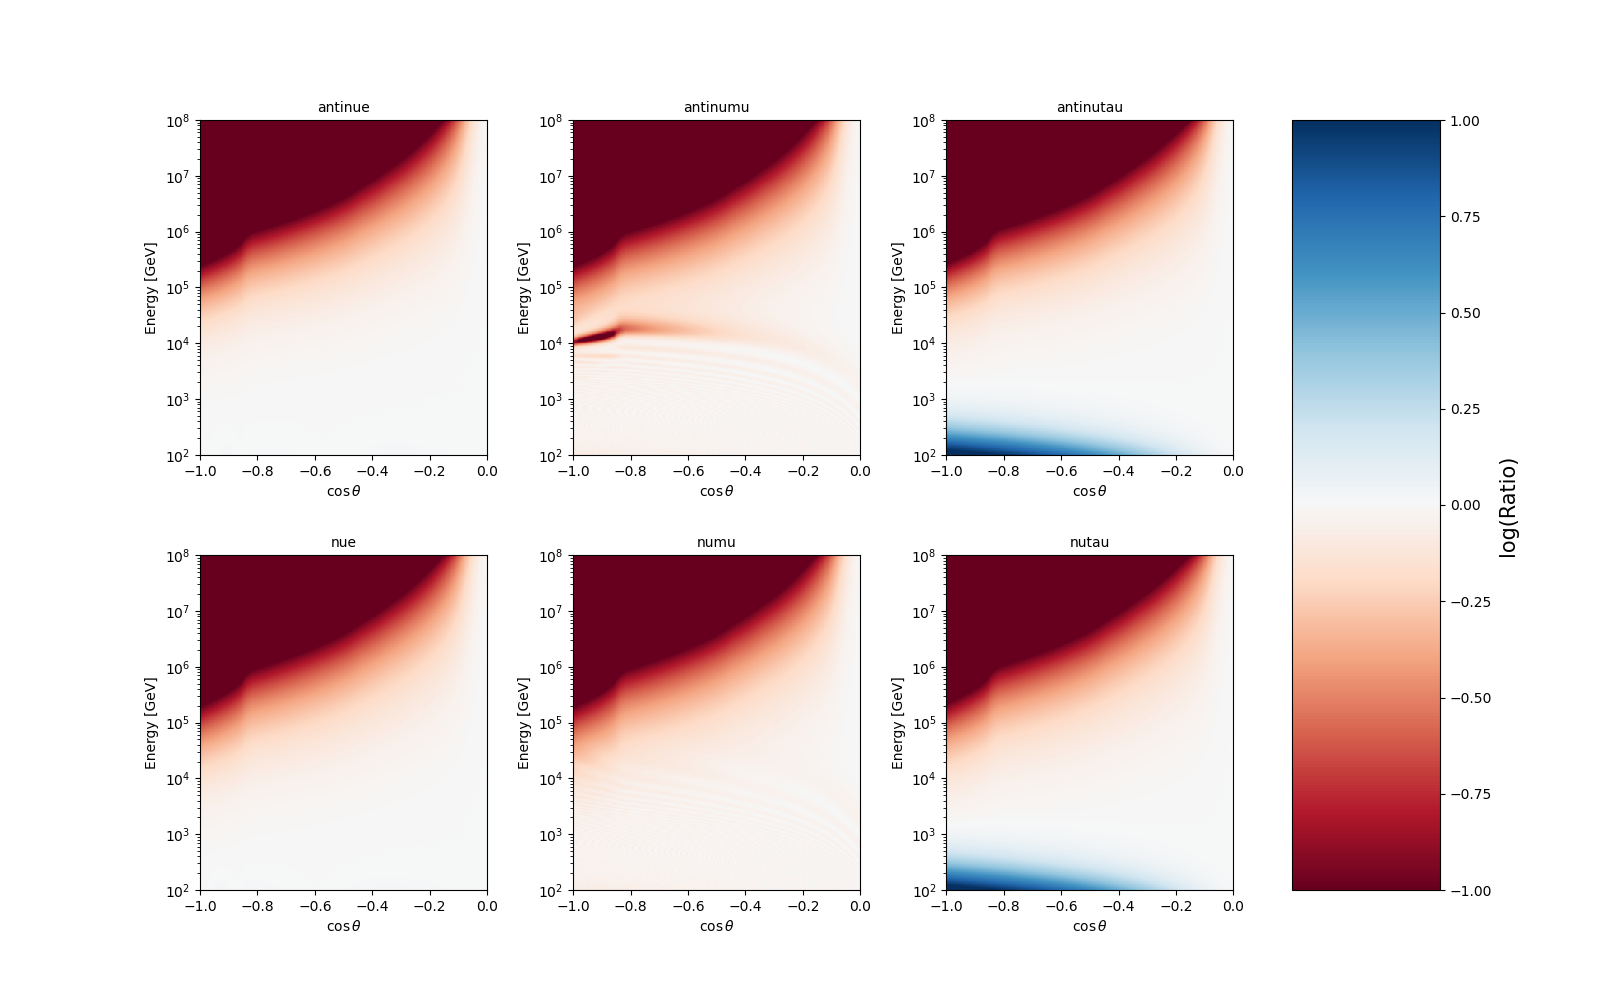
\includegraphics[width=0.8\linewidth]{figures/sterile_flux_plot.png}
    \caption{A plot showing the log of the ratio between the neutrino flux at the Earth's surface and at the IceCube detector. The top left corner of each panel shows the disappearance due to the Earth's opacity to high energy neutrinos. The blue region shows tau appearance from $3\nu$ oscillations. The resonance in the $\bar{\nu}_{\mu}$ channel is an example signature of eV$^{2}$-scale sterile neutrinos.}\label{fig:sterile_osc_sig}
\end{figure}

\subsection{Neutrino Propagation with Interactions}
In addition to neutrino oscillations and coherent matter effects, several other phenomena effect the full description of neutrino propagation through the Earth. 
These include, but are not limited to, neutrino flux attenuation as neutrinos interact in the Earth, the process where charged tau leptons produced through neutrino-nucleon interactions decay to produce lower energy tau neutrinos called tau regeneration, and Glashow resonance interactions~\cite{PhysRev.118.316}.
These effects become increasingly relevant at the higher energies relevant to the analysis presented in this dissertation.  
Here we describe the methods used for numerically propagating neutrino fluxes from the Earth's surface to IceCube; these procedures were originally described by Reference~\cite{arguelles2021nusquids}.

The neutrino flux is described as a function of energy $E$ and location $x$ for neutrino flavor $\alpha$ using the density matrix formalism in the weak-interaction flavor-eigenstate basis as 
\begin{equation}
    \rho(E,x) = \sum_{\alpha} \phi_{\alpha}(E,x) \ket{\nu_{\alpha}}\bra{\nu_{\alpha}},
\end{equation}
where $\phi_{\alpha}$ specifies the neutrino flux of the flavor $\alpha$. 
The evolution of the system can be described by the von Neumann equation,
\begin{equation}\label{eq:evol}
    \dfrac{\partial\rho (E,x)}{\partial x} = -i\left[ H(E,x), \rho(E,x)\right],
\end{equation}
where $H$ is the Hamiltonian for the whole system. 
$H$ can be approximated, in the case of small perturbations, as
\begin{equation}
    H(E,x) = H_{0}(E) + H_{1}(E,x)
\end{equation}
where $H_{0}$ is the term giving vacuum neutrino oscillations, which can be solved exactly, and $H_{1}$ is an additional term incorporating matter-effects.
These are, for neutrinos,
\begin{align}
    H_{0}(E) &= \dfrac{1}{2E} \left(\begin{array}{ccc} 0 & 0 & 0\\ 0 & \Delta m_{21}^{2} & 0 \\ 0 & 0 & \Delta m_{31}^{2}\end{array}\right)  \\
    H_{1}(E,x) &= \sqrt{2}G_{F} N_{e}(x) U_{PMNS}^{\dag} \left(\begin{array}{ccc}1&0&0 \\ 0 &0 & 0 \\ 0 & 0 & 0 \end{array}\right) U_{PMNS},
\end{align}
where $G_{F}$ is the Fermi constant, $U_{PMNS}$ is the PMNS neutrino mixing matrix, $N_{e}$ is the electron number density at position $x$, and the $\Delta m^{2}$ terms are the mass-squared splittings.  
Since the evolution of the vacuum component can be soled analytically, it is more convenient to evolve of the system in the interaction basis. 
So, we transform the density matrix and the mass-effect terms as 
\begin{align}
    \rho_{1}(E,x) &= e^{-i H_{0}x}\rho(E,x) e^{-iH_{0}x}. \\
    H_{I,1}(E,x)&= e^{-i H_{0}x} H_{1}(E,x) e^{-iH_{0}x}.
\end{align}
Similarly to Equation~\eqref{eq:evol}, the evolution in the interaction basis is dependent on the matter-effect term,
\begin{equation}\label{eq:mattermod}
    \dfrac{\partial_{1}\rho (E,x)}{\partial x} = -i\left[ H_{I,1}(E,x), \rho(E,x)\right].
\end{equation}
We require a series of additional terms that modify Eq~\eqref{eq:mattermod} to account for the effects which do not preserve neutrino number and energy. 
The first of which is the attenuation of the fluxes from neutrino-Earth interactions, which follow 
\begin{align}\label{eq:nu_evol}
    \Gamma(E,x) &= \dfrac{1}{2}\sum\limits_{\alpha\in(e,\mu,\tau)} \dfrac{\Pi_{\alpha}(E,x) }{\lambda_{NC}^{\alpha}(E,x) + \lambda_{CC}^{\alpha} (E,x)} \\
    \bar{\Gamma}(E,x) &= \dfrac{1}{2}\sum_{\alpha\in(e,\mu,\tau)} \dfrac{\bar{\Pi}_{\alpha(E,x)}}{\bar{\lambda}_{NC}^{\alpha}(E,x) + \bar{\lambda}_{CC}^{\alpha}(E,x) + \bar{\lambda}_{GR}^{\alpha}(E,x) }\label{eq:nubar_evol}
\end{align}
where $\Pi_{\alpha}$ is a neutrino projector onto the flavor $\alpha\in\left\lbrace e,\mu\tau\right\rbrace$, $\nu_{CC}^{\alpha}$ ($\nu_{NC}^{\alpha}$) is the charged (neutral) current neutrino interaction length given by $1/\left[ N_{nuc}(x)\sigma^{\alpha}_{CC(NC)}(E) \right]$~\cite{Formaggio:2013kya, Gandhi:1995tf, Beacom:2019pzs, Zhou:2019vxt, Cooper_Sarkar_2011}, and $\bar{\lambda}_{GR}^{e}$ is the mean free path due to the Glashow Resonance $1/\left[ N_{e}(x)\sigma^{e}_{GR}(E) \right]$~\cite{PhysRev.118.316}. 

We also account for tau regeneration, neutrino-antineutrino coupling, and low-energy neutrino re-injection from neutral current interactions following the functional forms for neutrinos $F$ and antineutrinos $\bar{F}$ given by 
\begin{equation}\begin{split}
    F\left[\rho,\bar{\rho}, E, x\right] &= \sum\limits_{\alpha} \Pi_{\alpha}(E,x)\int\limits_{E}^{\infty}\dfrac{\text{Tr}\left[ \Pi(E_{\nu_{\alpha}},x)\rho(E_{\nu_{\alpha}}, x) \right]}{\lambda_{NC}^{\alpha}(E_{\nu_{\alpha}}, x) } \dfrac{\partial N_{NC}^{\alpha}(E_{\nu_{\alpha}}, E)}{\partial E} dE_{\nu_{\alpha}} \\ 
    &+\Pi_{\tau}(E,x) \int\limits_{E}^{\infty}\int\limits{E_{\tau}}^{\infty} \dfrac{\text{Tr}\left[ \Pi(E_{\nu_{\tau}},x)\rho(E_{\nu_{\tau}}, x) \right]}{\lambda_{NC}^{\tau}(E_{\nu_{\tau}}, E) } \dfrac{\partial N_{NC}^{\tau}(E_{\nu_{\tau}}, x)}{\partial E} \\
    &\times \dfrac{\partial N_{dec}^{all}(E_{\tau}, E)}{\partial E} dE_{\nu_{\tau}}dE_{\tau} \\
    &+\left[ \text{Br}\left(\tau^{-} \to \bar{\nu}_{e}\right)\Pi_{e}(E,x)\int\limits_{E}^{\infty}\int\limits_{E_{\tau}}^{\infty} \dfrac{\text{Tr}\left[ \bar{\Pi}(E_{\nu_{\tau}},x)\bar{\rho}(E_{\nu_{\tau}}, x) \right]}{\bar{\lambda}_{NC}^{\tau}(E_{\bar{\nu}_{\tau}}, x) }\right.  \\
    &+ \left. \text{Br}\left(\tau^{-} \to \bar{\nu}_{\mu}\right)\Pi_{\mu}(E,x)\int\limits_{E}^{\infty}\int\limits_{E_{\tau}}^{\infty} \dfrac{\text{Tr}\left[ \bar{\Pi}(E_{\nu_{\tau}},x)\bar{\rho}(E_{\nu_{\tau}}, x) \right]}{\bar{\lambda}_{NC}^{\tau}(E_{\bar{\nu}_{\tau}}, x) } \right] \\
    &\times \dfrac{\partial \bar{N}_{CC}^{\tau}(E_{\bar{\nu}_{\tau}}, E)}{\partial E} \dfrac{\partial\bar{N}_{dec}^{lep} (E_{\tau}, E)}{\partial E} dE_{\bar{\nu}_{\tau}} dE_{\tau}
\end{split}\end{equation}
and 
\begin{equation}\begin{split}
    \bar{F}\left[\rho,\bar{\rho}, E, x\right] &= \sum\limits_{\alpha}\bar{\Pi}_{\alpha}(E,x)\int\limits_{E}^{\infty}\dfrac{\text{Tr}\left[ \bar{\Pi}(E_{\bar{\nu}_{\alpha}}, x) \bar{\rho}(E_{\bar{\nu}_{\alpha}}, x) \right]}{\bar{\lambda}_{NC}^{\alpha}(E_{\bar{\nu}_{\alpha} }, x)}\dfrac{\partial\bar{N}_{NC}^{\alpha}(E_{\bar{\nu}_{\alpha}}, E)}{\partial E} d E_{\bar{\nu}_{\alpha}} \\ 
    &+ \bar{\Pi}_{\tau} (E,x) \int\limits_{E}^{\infty}\int\limits_{E_{\tau}}^{\infty}\dfrac{\text{Tr}\left[ \bar{\Pi}(E_{\bar{\nu}_{\tau}}, x) \bar{\rho}(E_{\bar{\nu}_{\tau}}, x) \right]}{\bar{\lambda}_{NC}^{\tau}(E_{\bar{\nu}_{\tau} }, x)}\dfrac{\partial\bar{N}_{NC}^{\tau}(E_{\bar{\nu}_{\tau}}, E)}{\partial E} \\
    &\times \dfrac{\partial\bar{N}_{dec}^{all}(E_{\tau}, E)}{\partial E} dE_{\bar{\nu}_{\tau}} dE_{\tau} \\
    &+ \left[ \text{Br}\left(\tau^{+} \to \nu_{e}\right)\bar{\Pi}_{e}(E,x)\int\limits_{E}^{\infty}\int\limits_{E_{\tau}}^{\infty} \dfrac{\text{Tr}\left[\Pi(E_{\nu_{\tau}}, x)\rho(E_{\nu_{\tau}}, x) \right] }{\lambda_{NC}^{\tau}(E_{\nu_{\tau}}, x)}  \right. \\
    &+ \left.\text{Br}\left(\tau^{+} \to \nu_{\mu}\right)\bar{\Pi}_{\mu}(E,x)\int\limits_{E}^{\infty}\int\limits_{E_{\tau}}^{\infty} \dfrac{\text{Tr}\left[\Pi(E_{\nu_{\tau}}, x)\rho(E_{\nu_{\tau}}, x) \right] }{\lambda_{NC}^{\tau}(E_{\nu_{\tau}}, x)}  \right] \\
    &\times \dfrac{\partial N_{CC}^{\tau}(E_{\nu_{\tau}}, E)}{\partial E} \dfrac{\partial N_{dec}^{lep}(E_{\tau}, E)}{\partial E} dE_{\nu_{\tau}} dE_{\tau} \\
    &+\left(\sum\limits_{\alpha} \bar{\Pi}_{\alpha} (E,x)\right) \int\limits_{E}^{\infty} \dfrac{\text{Tr}\left[\bar{\Pi}_{e}(E_{\bar{\nu}_{e}}, x) \bar{\rho}(E_{\bar{\nu}_{e}}, x) \right]}{\bar{\lambda}_{GR}^{e} (E_{\bar{\nu}_{e}}, x)}  \\
    &\times \dfrac{\partial\bar{N}_{GR}^{e}(E_{\bar{\nu}_{e}}, E)}{\partial E} dE_{\bar{\nu}_{e}}
\end{split}\end{equation}

Interaction rates in these functionals for neutral current, charged current, and Glashow resonance interactions are given by 

\begin{align}
    \dfrac{\partial N_{NC(CC)}^{\tau} (E_{\nu_{\tau}}, E)}{\partial E} &= \dfrac{1}{\sigma_{NC(CC)}^{\alpha} (E_{\nu_{\alpha} })}\dfrac{\partial\sigma_{NC(CC)}^{\alpha}(E_{\nu_{\alpha}}, E_{\alpha})}{\partial E_{\alpha}}\hspace{0.5cm} \text{ and}, \\
    \dfrac{\bar{N}_{GR}^{e} (E_{\bar{\nu}_{e}}, E)}{\partial E} &= \dfrac{1}{\sigma_{GR}^{e}(E_{\bar{\nu}_{e}})} \dfrac{\partial\sigma_{GR}^{e}(E_{\bar{\nu}_{e}}, E_{e})}{\partial E}.
\end{align}
The tau decay distributions for the leptonic-only modes ($N_{dec}^{lep}$) and for all-modes ($N_{dec}^{all}$) are given by 
\begin{align}
    \dfrac{\partial N_{dec}^{lep}(E_{\tau}, E)}{\partial E} &= \dfrac{1}{\bar{\Gamma}_{lep}^{\tau}(E_{\tau})} \dfrac{\partial\bar{\Gamma}_{lep}^{\tau}(E_{\tau},E)}{\partial E} \\
    \dfrac{\partial N_{dec}^{all}(E_{\tau}, E)}{\partial E} &= \dfrac{1}{\bar{\Gamma}_{all}^{\tau}(E_{\tau})} \dfrac{\partial\bar{\Gamma}_{all}^{\tau}(E_{\tau},E)}{\partial E} 
\end{align}

These systems are implemented within the \texttt{nuSQuIDS} framework~\cite{arguelles:2015nu, arguelles2021nusquids}, which implements Equations~\eqref{eq:nu_evol}-\eqref{eq:nubar_evol} to numerically propagate the state-density matrix along a neutrino fluxes' baseline. 
Different neutrino oscillation parameters can be specified, along with various other new physics scenarios, if desired.

\section{Structure}

In this dissertation I present the work for and the results from a multichannel search of signatures of matter-enhanced neutrino oscillations with eV$^{2}$-scale sterile neutrinos. 
It is organized as follows:

\textbf{Chapter \ref{chapter:intro}} has introduced the background physics relevant for this work and the sterile neutrino model we are testing.

\textbf{Chapter \ref{chapter:icecube}} will describe the IceCube Neutrino Observatory and the details of its operation. 

\textbf{Chapter \ref{chapter:degg}} will describe the upcoming IceCube Upgrade and ongoing work being done to test the new optical modules.

\textbf{Chapter~\ref{chapter:sense}} will provide the calculations for the predicted sensitivities for this analysis~\cite{PhysRevD.105.052001}. 

\textbf{Chapter \ref{chapter:gen}} will discuss the event generation schema and Monte Carlo simulation procedure used in IceCube~\cite{ABBASI2021108018}.

\textbf{Chapter~\ref{chapter:unc}} will summarize the sources of systematic uncertainty relevant for this analysis.

\textbf{ Chapter~\ref{chapter:res}} will finally provide the results of this analysis. 

Chapter entries with citations refer to the papers in which the work discussed was published.



\end{document}
